\ofsubsection{Maria \& Draco}
%
\ofquote{"The West and East were waging war.
Draco, the West's great hero, thinks of his love, Maria.
Is she safe? Is she waiting?
The forces of the West fell, and Maria's castle was taken.
Prince Ralse, of the East, took her hand by force. But she never stopped 
yearning for Draco..."\\}{Excerpt from opera "Maria \& Draco"}
%
\vfill
%
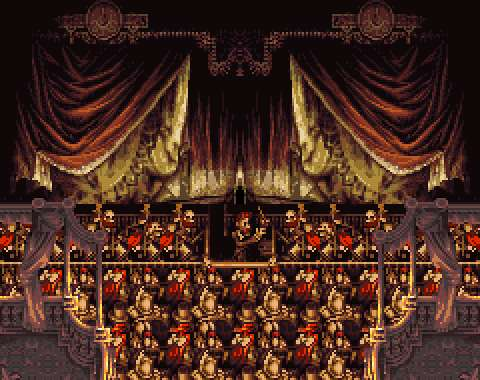
\includegraphics[width=\columnwidth]{./art/mariaanddraco/opera.jpg}
%
\vfill
%
\accf{Maria \& Draco} is a prepared adventure that can be completed in a single session and is designed for a party of Level~3 characters.
Their stories of the protagonists should explain why they are presently staying at the wealthy city Jidoor.
In this adventure, the party is tasked with preventing the kidnapping of a famous opera singer.
%
\vfill
%
\ofquote{"This is simply horrid! I want the performance to be a success! But I don't want Maria to be abducted!"\\}{Impresario}
%
\vfill
%
While resting at the city of Jidoor, the adventurers meet the owner of the town's opera house, he calls himself "Impresario".
He is an older, well-dressed man who is in constant worry about the upcoming opera called "Maria \& Draco".
Impresario is desperately looking for security guards for tomorrow's opera performance.
He offers 1000G to the party for handling the job, which they accept, despite not being paid up front.
At the morning of the opera, they meet Impresario at the opera house.
As they enter, he is running around frantically and upon noticing the party, he immediately hands them the following letter.\\
%
\vfill
%
Dearest Maria,\vspace{0.6cm}\\
I have decided to take you as my wife, so I'll be coming to kidnap you.\vspace{0.6cm}\\
\hspace*{0.5cm}The Wandering Gambler\\
%
\newpage
%
After he has calmed down, Impresario explains that the "Wandering Gambler" is a man named Setzer Gabbiani, who has caused trouble to him in the past.
He further describes Setzer as "a gambling vagabond who finds freedom from society's narrow views of morality aboard his airship" in a sarcastic tone.
Impresario also explains that Maria is the star of the show, so her safety is of utmost importance.
He proposes the following plan to keep her safe: one of the party members should play the role of Maria and act as a decoy.
He expects Setzer to make his move at the end of the first scene and try to abduct Maria onto his airship, but if he kidnaps the decoy, they can confront him instead.
He suggests that the decoy should carry a rope, so he or she can pull up the rest of party onto the airship if necessary.
The party may suggest other ideas as well, but Impresario will not accept any plan that might put the real Maria in danger.
If the party accepts his plans, they have to choose one of their own to play Maria's part in the opera, henceforth that character will be referred to as "Maria".
%
\vfill
%
\ofquote{"W...wait! I'm a GENERAL, not some opera floozy!"\\}{Celes}\\\\
%
Impresario will show them Maria's room, where "Maria" can get dressed and practice for her part.
"Maria" has to look as similar to the original as possible, who is a short, blond haired women in a long white dress.
Accordingly, the party might have to buy a new dress and wig or get creative in other ways, they can convince Impresario to cover additional costs. 
They are free to explore the town to shop or make other preparations until the evening. 
"Maria" should practice the following script for her part in the first scene:
%
\vfill
%
Maria enters the stage.\vspace{0.2cm}\\
"Oh my hero, so far away now. Will I ever see your smile?"\vspace{0.2cm}\\ 
"Love goes away, like night into day. It's just a fading dream."\vspace{0.2cm}\\ 
"Our love is brighter than the sun. For eternity, for me there can be, only you, my chosen one."\vspace{0.2cm}\\ 
Maria picks up the flowers, climbs the stairs to the balcony high atop the castle, then raises the flowers to the stars.\vspace{0.2cm}\\
"We must part now. My life goes on. But my heart won't give you up."
%
%
\vfill
%
During the opera, "Maria" first appears at the end of the first scene, where she has to perform the above mentioned part.
You as the GM have to rate "Maria's" performance on a scale from 1 to 10.
Below is a list of criteria, which you can use to award points.
You should keep the rating secret at this point, but you can to already give a hint by narrating the reaction of the audience.
%
\clearpage
%
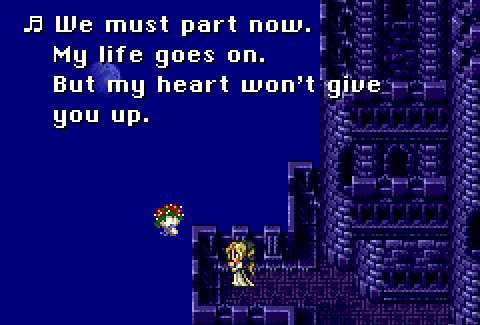
\includegraphics[width=\columnwidth]{./art/mariaanddraco/maria.jpg}\\
%
\vfill
%
\ofbullet{1 point for each line that the player correctly recites, so up to 4 points.}
\ofbullet{1 bonus point, if the player makes an attempt to actually sing the lines.}
\ofbullet{Up to 3 points depending on how much effort the party has spent on making "Maria" actually look like Maria.}
\ofbullet{1 point if the player remembers to pick up the flowers, walk up the stairs and raise the flowers up.}
\ofbullet{The player makes a DC~8 to determine whether his or her character manages to present themselves as gracefully as the real Maria. If the check succeeds, award another 2 points. The DC can be lower if "Maria" has any performance related experience.}
%
\vfill
%
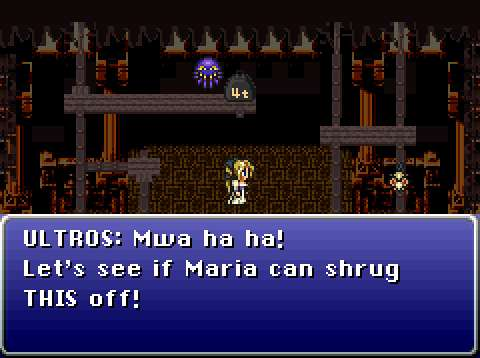
\includegraphics[width=\columnwidth]{./art/mariaanddraco/ultros.jpg}
%
\vfill
%
As Maria's part is playing out on the stage, Impresario and the party are watching from their lodge seats.
Suddenly, Impresario notices something on the catwalk: someone, or rather something, is trying to push an anvil down onto the stage!
The party recognizes that it is the strange octopus named Ultros who is behind the plan.
The adventurers have met Ultros before and have beaten him, so he wants to take revenge by sabotaging the opera. 
Impresario starts to panic and begs the party to stop Ultros's plan.
He points them to a room on the right hand side of the lodge and tells them to pull the rightmost lever.
%
\newpage
%
\ofquote{"Silence! You are in the presence of octopus royalty! A lowborn thug like you could never defeat me!"\\}{Ultros}\\\\
%
After they move out of their seats, each party member has to make a DC~6 check to decide whether they disturb the audience.
If at least one of them fails, deduct one point from the performance.
Once in the room, the party notices four levers on the wall.
The rightmost lever opens a pathway to the catwalk, the other ones have the following effects and pulling either one deducts a point from Maria's performance: lever 1 makes a sound like a barking dog, lever 2 turns off the lights in the opera hall and lever 3 opens up a trap door below the player who pulled the lever, which lets him or her slide directly onto the stage. 
Once the party enters the catwalk, they see that Ultros is just about to drop the anvil on "Maria".
As they move closer, the fragile planks of the catwalk fail to support their combined weight and both the party and Ultros
fall down onto the stage.
"Maria" has to make a DC~7 check and if she fails, she falls unconscious, otherwise she can participate in the ensuing battle.   
The ones who fell, including Ultros, take 1d damage, but they can immediately get up to start the fight!
%
\vfill
%
\ofmonster{Ultros}{3}{
\includegraphics[width=0.32\columnwidth]{./art/mariaanddraco/ultrosmon.jpg}}
{
	HP: & \hfill 60 & MP: & \hfill 90 \\
	STR: & \hfill 4 & DEF: & \hfill 2 \\
	MAG: & \hfill 1 & RES: & \hfill 3 \\
	AGI: & \hfill 2 & Size: & \hfill L\\
}
{\accf{Ink}: 1d DMG, 3u Range \hfill \accf{Drops:} 500G\\
\accf{Immune}:\poison\sleep\blind\immobile \hfill \accf{Final Attack, Dual Attack}
}
{	
	\mspell{Water}{6}{0r}{Single}{4u}{You deal 2d water damage to the target.}{\water}
	\mtech{Acid Rain}{8}{0r}{3u}{Self}{
		All enemies in the target area suffer 2d water damage.
		In addition, all affected targets make a DC~7 check and suffer Poison for 1 round upon failure 
	}{\poison\water}	
	\mtech{Tentacle}{4}{0r}{2u (front)}{Self}{Deal 2d damage to all enemies in the target area.}{}	
	\mpassive{Blindtouch}{Every target that rolls below 6 on an evasion check against your Attack, suffers Blind for 3 rounds.}{}		
}
%
\vfill
%
After the party defeats Ultros, they hear a voice loudly exclaiming: "What a performance!".
Suddenly, a man descends onto the stage using a grappling hook.
The man is of course none other than Setzer.
He quickly grabs "Maria" and activates the device once more to pull himself back up to the lodge with "Maria" in his arms.
From there he escapes to his airship, which is waiting right above the rooftop of the opera house.
The party tries to follow him but they have to take a longer route to reach the the roof.
As they arrive at the rooftop, Setzer is just getting ready to take off with the airship.
%
\clearpage
%
\ofquote{"Nothing to lose but my life..."\\}{Setzer}\ofpar
%
%
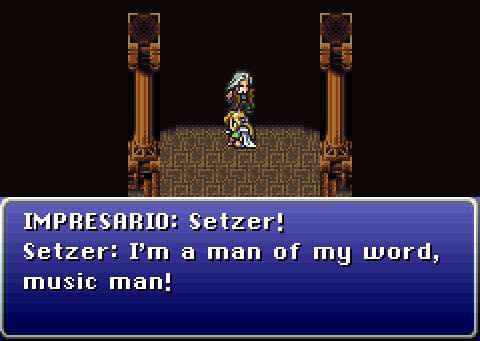
\includegraphics[width=\columnwidth]{./art/mariaanddraco/setzer.jpg} 
%
\\\\
%
He locks "Maria" in his cabin and gets on deck to start the engine.
If "Maria" fell unconscious before, she will now wake up and realize that Setzer has abducted her.
If everything went according to plan up to this point, she should have a rope with her.
She can let it out of one of the windows in this room and the party can reach from the roof. 
Optionally, you can ask each player to perform a DC~7 check to decide whether they are able to successfully grab and climb the rope.
After gaining some distance on the opera house, Setzer returns to the cabin.
Upon taking a closer look at "Maria" and noticing the rest of the party, he understands that he has been tricked and becomes angry.
The course of this confrontation depends on the decisions the party makes.
Below are some general ideas on roleplaying as Setzer, but you can, or might have to, improvise some aspects of this section.
%
\ofpar
%
\accf{The party tries to solve the conflict peacefully:}\\
Setzer is generally open to this as he realizes that he is outnumbered.
He can be convinced to let the party go and to stay away from the opera house in the future.
He is also open to joining the party, if they offer him the prospect of exciting future adventures.
Setzer is much easier to convince if the arrangement involves gambling of any sort, which he loves.
If the party tries to trick him, for example with a rigged coin toss, he will show even more respect.
However, he does not accept any deal that involves him being restrained or handed over to the authorities.
%
\ofpar
%
\accf{The party tries to kill or restrain Setzer forcefully:}\\
For this case, Setzer's combat statistics are listed below.
Despite being outnumbered, he does not give up easily and does not hesitate to use dirty tricks to get the upper hand.
If the party manages to defeat Setzer, they can decide whether they want to let him live or restrain him to deliver to the authorities.
Either way, they will need to maneuver and land the airship.
The player that takes control of the airship has to perform a check with a DC that can vary between 6 and 8, depending on the character's proficiency in handling vehicles.
If he or she fails the check, the ship crashes near Jidoor and gets destroyed.
All passengers on board survive, but everyone suffers 2d damage.
%
\vfill
%
\ofmonster{Setzer}{4}{
\includegraphics[width=0.25\columnwidth]{./art/mariaanddraco/setzermon.jpg}}
{
	HP: & \hfill 40 & MP: & \hfill 80 \\
	STR: & \hfill 2 & DEF: & \hfill 1 \\
	MAG: & \hfill 0 & RES: & \hfill 1 \\
	AGI: & \hfill 4 & Size: & \hfill M\\
}
{
\accf{Cards}: 2d DMG, 3u Range \hfill \accf{Auto-Haste}
}
{
	\mtech{Slots}{8}{0r}{?}{?}{
		Roll 1d. One of the following effects occurs depending on the result:
		On a 1 or 2, the area within 3u of you is filled with smoke until the start of your next turn. 
		Everyone inside it, suffers Blind, but gains Blink.
		On a 3 or 4, you teleport to a location of your choice within 3u.
		On a 5 or 6, an explosion deals 2d fire damage to all enemies within 2u.
	}{}	
	\mtech{Gil Toss}{4}{0r}{2u}{5u}{You throw 100G to deal 2d damage to all enemies in the target area.}{}
	\mtech{Vanish}{8}{0r}{Single}{Weapon}{You become invisible for up to 5 rounds or until you take an action. While invisible, you gain Blink. Also, if you hit an Attack while invisible, you automatically score a Critical Hit.}{\blink}	
	\mreaction{Fixed Dice}{Whenever you roll for a check or to determine damage, you can re-roll one die that has the result~1.}{}		
}
%
\vfill
%
After dealing with Setzer, the party can return to the opera house to collect their reward.
Impresario considers their contract fulfilled if they have managed to drive away Setzer.
First, every party member gains a \accf{Level Up}!
In addition, they receive a reward depending on the rating of Maria's performance:\\\\
\ofbullet{\accf{1-3 points:} despite driving away Setzer, the opera performance was a disaster, leaving the audience deeply unsatisfied. Impresario blames the party for being sloppy and halves his originally offered reward to 500G.}\\\\
\ofbullet{\accf{4-6 points:} despite some hick ups, the performance went well overall. Impresario is satisfied and hands the party 1000G as agreed upon.}\\\\
\ofbullet{\accf{7-10 points:} the party managed to amaze the audience with an outstanding performance. Impresario is thrilled and doubles the originally agreed reward to 2000G.}
%
\clearpage